\documentclass[10pt]{article}
\usepackage[a4paper,margin=1in]{geometry}
\usepackage{fontspec,graphicx,xurl,booktabs,array,needspace}
\setmainfont[Path={fonts/},BoldFont=timesbd.ttf,ItalicFont=timesi.ttf,BoldItalicFont=timesbi.ttf]{times.ttf}
\urlstyle{same}
\makeatletter\renewcommand\normalsize{\@setfontsize\normalsize{10}{12}}\makeatother
\let\small\normalsize\let\footnotesize\normalsize\let\scriptsize\normalsize
\let\large\normalsize\let\Large\normalsize\let\LARGE\normalsize
\let\huge\normalsize\let\Huge\normalsize
\setlength{\parindent}{0pt}\setlength{\parskip}{3pt}
\setlength{\emergencystretch}{2em}
\let\originalsection\section
\renewcommand\section{\Needspace{6\baselineskip}\originalsection}
\begin{document}\normalsize

\begin{center}\textbf{CARDIODIAG: Supplementary Methods and Numerical Traceability}\end{center}
Editorial integration: 15 November 2026. Evidence baseline: \path{97ee42c4d79453ef346bc0cfcb62e87fdfb7223b}.
This supplement reconciles the reviewed submission draft with all final analyses. It reports saved evidence, not a new experiment or an independent investigator replication. All numbers are traceable to the repository; the reviewed package's unsupported additional 1,500-draw bootstrap is not imported.

\section*{S1. Cohorts, endpoints and experimental unit}
ZAS contains 303 source rows, 216 Cad and 87 Normal labels. Its provider workbook and validated CSV agree on 55 non-target fields plus Cath, although provider prose refers to 54 predictors. Exact duplicate checks and file reconciliation do not establish unique patients: verified person IDs, longitudinal linkage and predictor timestamps are unavailable. The statistical unit remains the source record.

AngioCAD has 413 label IDs and 377 matching clinical records; 36 label-only records are excluded from clinical-feature modeling. Of 377 matched cases, 298 have at least one of 15 segments in a category above 50\% stenosis and 79 do not. Ten of the 79 have a 26--50\% category. Source catalogue threshold $\geq50\%$ and target categories $>50\%$ cannot be fully harmonized from these files. Non-positive target records are not healthy population controls. The matched referral spectrum includes 186 STEMI, 20 NSTEMI, 55 unstable-angina and 116 stable-angina cases. Six ages and 46 smoking values are missing. Exact clinical coding equivalence and acquisition timing remain unresolved.

Primary target results retain the 377-case rule. Excluding ten boundary cases leaves 367 records and 298 positives; upper assignment retains 377 records and makes 308 positive. These are scoring sensitivities, not recovered ground truth. Source-only training and subsequent target-label updating are distinct tasks.

\section*{S2. Related literature and distinguishing scope}
\textbf{Khan et al., CardioDiag (2026).} The original work contributes XAI-guided dimensionality reduction and optimized voting/stacking. Those architectures and explanations are prior work. Our study does not claim an OVEC/OSEC head-to-head win. Primary record: \url{https://doi.org/10.7717/peerj-cs.4059}.

\textbf{Mansoor, Chettri and Naleer (2024).} Machine/deep-learning CAD comparisons illustrate established model-search work on the Alizadeh Sani resource. The present contribution is paired information matching and probability-construction traceability, not source-cohort novelty. Primary record: \url{https://pubmed.ncbi.nlm.nih.gov/39031414/}.

\textbf{Baratpur et al. (2025).} Bayesian-optimized SVM, feature selection, resampling and explanatory analyses precede this study. Their scores cannot be ranked against ours without identical data, information and assessment rules. Primary record: \url{https://pubmed.ncbi.nlm.nih.gov/41458563/}.

\textbf{Elemam, Refaat and Makhlouf (2026).} SHOW combines SHAP ranking and wrapper feature selection on public CAD resources. Feature selection and interpretability alone are therefore not new contributions here. Primary record: \url{https://pubmed.ncbi.nlm.nih.gov/41882033/}.

\textbf{Hosseini et al., AngioCAD (2026).} The provider article describes a public angiography resource and an adaptive fusion framework. This study uses its clinical-feature and stenosis workbooks for a separate shared-core transfer analysis; it does not reproduce the video framework. Primary record: \url{https://pubmed.ncbi.nlm.nih.gov/42033972/}. Dataset: \url{https://doi.org/10.5281/zenodo.15826856}.

\textbf{Methodological context.} Cawley and Talbot address selection bias; Van Calster et al. address calibration; Riley et al. address external evaluation and precision-based sample size; TRIPOD+AI and PROBAST+AI guide reporting and risk-of-bias appraisal. These established tools are applied, not invented, in CARDIODIAG. The literature check is targeted rather than systematic and does not prove priority. A five-year prognostic/polygenic cohort is not a numerical comparator for retrospective Cath labels, so that tangential reference from the reviewed package is not added to the main manuscript.

\section*{S3. Information sets and selected procedures}
The eligible source group has 38 fields: seven risk, ten symptom/examination, seven ECG and fourteen laboratory variables. Cath, EF-TTE, Region RWMA and VHD are excluded from this predictor group. Exclusion does not establish correct pre-decision timing for retained fields. The five-core transfer allowlist is Age, Sex, DM, HTN and Current Smoker. It differs from the historical V3 information set and is not a transported 38-field model.

Fifteen source outer partitions comprise three repeats of five folds. Each procedure produces 303 out-of-fold predictions per repeat. Repeats reuse the same rows and overlapping development data: 909 procedure predictions are not 909 independent patients. Historical selection evaluates six groups and five unique families, 30 group-family candidates and 120 settings, using inner AUC. All transforms are fitted inside the relevant training subsets.

The equal-information L2 control uses all 38 fields and C in 0.1, 1 and 10. Fixed-family controls use 28 fields without symptoms/examination and 17 risk-plus-symptom fields. Historical post-selection sigmoid calibration is retained for matching, but its calibration labels influence configuration selection and its inner-fit/full-refit sizes differ. Thus these are information-matched procedures, not identical pipelines differing only in classifier complexity.

For independent calibration, each outer-training set is partitioned into development and calibration records three times. The complete search is rerun only in development; the exact fitted base model scores the disjoint calibration block and outer test. The fitted map is retained without swapping in a larger refit base model. Raw and calibrated ensembles average the same three components. Only that matched contrast isolates the calibration operation. The weak raw-probability sigmoid uses C=$10^6$; version two evaluates offset-only, fixed-C1 logit and inner-calibration-CV logit maps on the same frozen components.

\section*{S4. Robustness and uncertainty boundaries}
The version-two typed schema distinguishes 17 continuous, one ordinal, eleven numeric-binary and nine nominal fields. Its mean AUC/Brier 0.899248/0.112920 is worse than historical full38 L2 0.917447/0.101124. It remains unpromoted. The optional estimator adds a 20\%-masked training copy, half weighting each original/copy and fitting indicators inside every estimator fit. Copies never cross into validation. At 50\% MCAR deletion it improves AUC 0.687544 to 0.703322, but clean-input AUC drops 0.805884 to 0.804465. Whole-block scenarios also show trade-offs; MCAR results do not establish robustness to clinical MNAR missingness.

The paired 1,000-draw source bootstrap shares resampled record IDs across repeats and conditions on saved fits. Fixed-C1 minus identical raw Brier bounds are approximately $[-0.005329,0.000685]$, spanning zero. The 2,000-draw fixed-target bootstrap does not refit source models. Fifty typed-L2 out-of-bag refits assess that pipeline, not the full search. Final five-core coefficient bootstraps are another 50 refits, using grouped duplicate copies in C tuning. These distinct analyses must not be merged into a patient-level or full-search confidence claim.

Prespecified age/sex subgroup diagnostics use repeat one and flag fewer than ten records in either outcome class as unstable. They are not fairness certification. Joint calibration intercept/slope is distinguished from intercept-only updating with slope fixed at one. AP reflects the high event prevalence; Brier is mean squared probability error, not Brier skill.

\section*{S5. Final analyses retained from the latest release}
Training-only nested out-of-fold scores set a 90\%-sensitivity threshold in each outer development set. Held-out sensitivities are 0.879630, 0.888889 and 0.898148; mean specificity is 0.490421. Mean PPV/NPV are 0.812574/0.640008 in this enriched source cohort. No clinical threshold or community-screening predictive value is inferred.

Source learning curves retune C within stratified 25/50/75/100\% outer-training subsets, leaving the same outer tests untouched. Mean AUC grows from 0.769024 to 0.805884. Target offset-learning curves fit on 10/25/50/75/100\% of adaptation folds, disjoint from evaluation cases. Brier is 0.152489 at 10\% and 0.150723 at 100\%. A single deterministic stratified sample per fraction/fold does not establish a required adaptation sample size.

Five-percent independent binary code flips reduce mean AUC to 0.782842 and increase Brier to 0.161284; five-year age rounding retains AUC 0.805467. These are numerical scenarios, not measured clinical error distributions. Decision curves retain a fixed research grid 0.05--0.95 and explicit all/none strategies. Without an intended action and elicited harm ratio, apparent net benefit is exploratory rather than evidence of clinical effectiveness.

\section*{S6. Exact paths and executable traceability}
All following paths are repository-relative. Long paths are shown on separate lines so they wrap without colliding with another table column.

\textbf{Original source runner:}\par\path{CARDIODIAG_FRESH/runner/research_extension_v1/zas.py}
\par\textbf{Source probability evidence:}\par\path{CARDIODIAG_FRESH/results/research_extension_v1/zas/PREDICTIONS.csv}
\par\textbf{Transport runner:}\par\path{CARDIODIAG_FRESH/runner/research_extension_v1/transport.py}
\par\textbf{Frozen target scores:}\par\path{CARDIODIAG_FRESH/results/research_extension_v1/transport/TARGET_PREDICTIONS.csv}
\par\textbf{Version-two runner:}\par\path{CARDIODIAG_FRESH/runner/research_extension_v2/run.py}
\par\textbf{Calibration maps/predictions:}\par\path{CARDIODIAG_FRESH/results/research_extension_v2/CALIBRATION_PREDICTIONS.csv}
\par\textbf{Target updating:}\par\path{CARDIODIAG_FRESH/results/research_extension_v2/ADAPTATION_PREDICTIONS.csv}
\par\textbf{Final exploratory runner:}\par\path{tools/finalize_analyses.py}
\par\textbf{Final evidence namespace:}\par\path{CARDIODIAG_FRESH/results/final_analyses_v3/}

\textbf{Paper numerical reconstruction:}\par\path{tools/paper_evidence.py}
\par\textbf{Generated per-repeat metric trace:}\par\path{CARDIODIAG_FRESH/paper/final/NUMERIC_TRACEABILITY.csv}
\par\textbf{Figure source hashes:}\par\path{CARDIODIAG_FRESH/paper/final/FIGURE_INPUTS.json}
\par\textbf{Paper/source/artifact hashes:}\par\path{CARDIODIAG_FRESH/paper/final/PAPER_EVIDENCE_MANIFEST.json}

\section*{S7. Reproduction and scope of verification}
Use Python 3.11 and the pinned release requirements. Execute these commands from the repository root:
\begin{quote}\raggedright
\path{python tools/portable_release.py --root . --check-runtime}\par
\path{python tools/verify_reliability_v2.py}\par
\path{python tools/verify_final_analyses.py}\par
\path{python tools/paper_evidence.py}\par
\path{python tools/verify_publication.py --root .}\par
\path{python -m pytest -q}
\end{quote}
The checks reconstruct original, version-two and final metrics and validate memberships/hashes. They do not independently refit all 30-candidate jobs. The figure builder reads the reconstructed CSV and frozen prediction/summary files. No literal metric arrays from the reviewed package or additional unsupported bootstrap bounds are used. Versioned manifests retain experiment code and data inputs; the editorial artifact manifest separately records this paper build.

\clearpage\section*{S8. Figures derived from frozen evidence}
These figures show complete-repeat means only, with no implied population confidence intervals. They accompany the main paper's ROC, learning and decision-curve overview. All labels use Times New Roman at nominal 10 points. Source metric files and hashes are listed in the numerical trace and figure manifest.
\par\noindent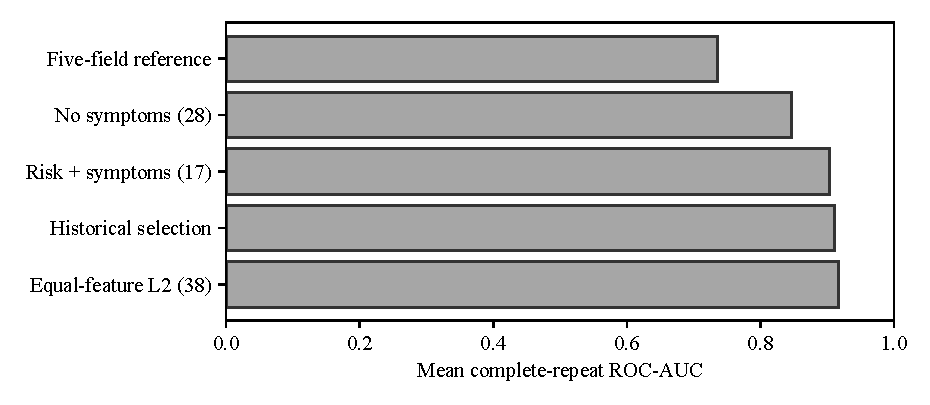
\includegraphics[width=\linewidth]{SOURCE_COMPARISON.pdf}
\par Source comparisons use distinct information sets. The automated search is not an OVEC/OSEC head-to-head comparison.
\par\noindent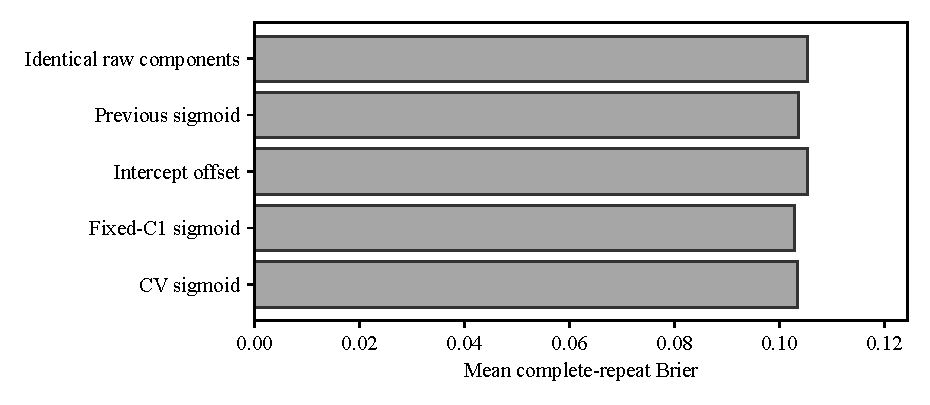
\includegraphics[width=\linewidth]{CALIBRATION_LOSS.pdf}
\par The calibration comparison retains identical base components; lower Brier is better. Differences remain conditional on the saved fits.
\clearpage
\par\noindent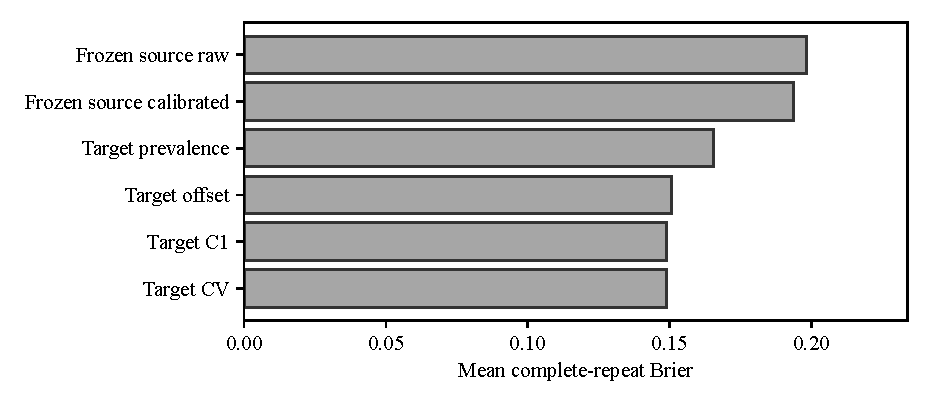
\includegraphics[width=\linewidth]{TARGET_LOSS.pdf}
\par Source-frozen and target-label-updated arms differ in information used for fitting. Label-assisted updating is not untouched external validation.
\par\noindent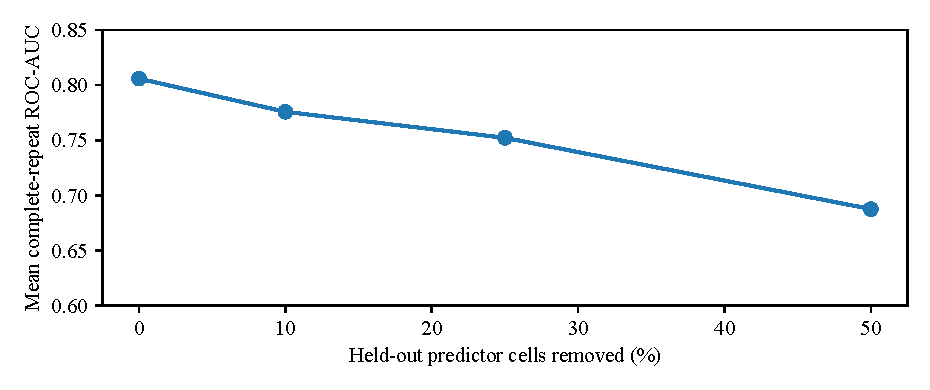
\includegraphics[width=\linewidth]{MISSINGNESS_STRESS.pdf}
\par Input deletion reuses fixed masks and source fits. Random deletion does not represent all clinical missingness mechanisms.

\end{document}
